\chapter*{SYSTEM ARCHITECTURE AND DESIGN}
\thispagestyle{fancy}
\addcontentsline{toc}{chapter}{SYSTEM ARCHITECTURE AND DESIGN}

\section*{What is a Subcontext?}
\addcontentsline{toc}{section}{What is a Subcontext?}
A \textit{subcontext} is best understood as a snapshot of a process’s virtual memory, frozen in time and made executable within the virtual address space of another process. In abstract terms, a subcontext is a context within a context: a self-contained non-contiguous subset of regions that can be mapped into and invoked by a host (client) process without mutual interference. The process into which the subcontext is mapped is called the \textit{host} or \textit{client process}, while the mapped subcontext resides as a passive region within its virtual memory. Our system views the client process as its own trivial subcontext, although it is never serialized into an image file or shared with another process.

A subcontext is created when a process, using the server-side library, serializes selected regions of its memory into an \textit{image file}. This file includes the binary content of executable code, static data, and most importantly, function pointers that form the subcontext's interface. After serialization, the original process may terminate safely. From that point onward, the subcontext exists independently in the form of a mutable image file.

The mutability of the image file affects the system thusly: suppose client processes A and B map in an image file as a subcontext which serializes a process that maintains a global counter as well as a function which increments the counter. When client process A executes this function, the subcontext's global counter, and therefore memory, has been modified. When client process B now executes this function, they will find the value of the counter to be the modified value left by client process A, instead of the counter's original value. Speaking from a more technical perspective, as writes occur to pages in the shared subcontext, these writes are written to the backing file both implicitly and lazily.

This design makes shared subcontexts possible, but does incur the question of race conditions. Simply put, this is not something we explored in the development of this system, but certainly merits exploration in the future. The intent is that the mapped subcontext is essentially multi-threaded across the processes which have mapped it into their memory. 

While mapped subcontexts remain isolated from one another, unaware of adjacent subcontexts mapped into the same client process, our intention was to allow them to read from and write to the memory of the client process in order to provide system services. Again, this is not something we had the time to explore in our prototype but is something that we would like to touch on in future.

Technically, a subcontext consists of a set of virtual memory pages, with disjoint address ranges, both among themselves and relative to any memory already used by the client. The locations at which subcontext pages are mapped are fixed and do not change throughout the life of a subcontext. These pages are mapped into unused virtual memory regions of the client process, allowing for safe execution of subcontext routines without the risk of overlapping or clashing with the client’s own memory layout.

\subsection*{The Lifecycle of a Subcontext}
\addcontentsline{toc}{subsection}{The Lifecycle of a Subcontext}
\begin{itemize}
    \item \textbf{CREATION}: A server process picks up the server-side library and uses its functionality to serialize selected regions of its memory and store them in an image file.
    \item \textbf{PERSISTENCE}: The image file contains and represents the subcontext and may persist long after the server process terminates.
    \item \textbf{MAPPING}: A client process picks up the client-side library and uses its functionality to map the subcontext from an existing image file into its virtual address space.
    \item \textbf{EXECUTION}: The client process invokes functionality from the mapped subcontext, using entry points well-defined by the subcontext itself.
    \item \textbf{UNMAPPING/TERMINATION}: The subcontext remains mapped in the virtual address space of the client process until it is either explicitly unmapped or the client terminates.
\end{itemize}

This lifecycle model supports sharing, reuse, and concurrency. Clients remain isolated from one another, and each subcontext mapping is private to the client process that owns it.


\begin{figure}[ht]
    \centering
    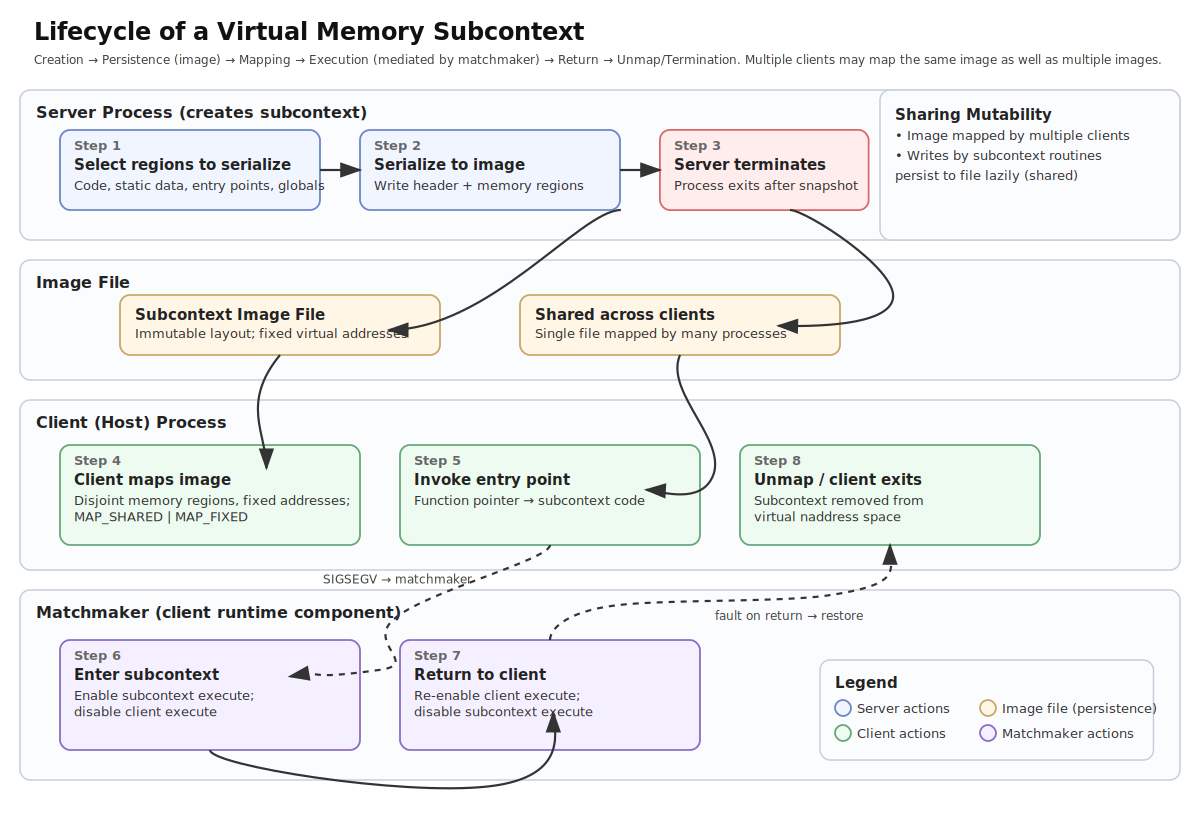
\includegraphics[width=\textwidth]{subcontext_lifecycle.png}
    \caption{The lifecycle of a subcontext.}
\end{figure}


\subsection*{Memory Topology and Placement}
\addcontentsline{toc}{subsection}{Memory Topology and Placement}
Subcontexts are mapped into the address space of a client process at fixed locations, which makes mapping impossible if overlapping mappings already exist. Once placed, subcontext pages are immobile—meaning they are fixed at their mapped addresses to preserve pointer validity and layout expectations.

We assume that modern systems offer sufficiently large and sparsely used virtual address spaces to allow this strategy to scale. The pinned placement avoids the need for complex relocation or dynamic symbol resolution.

A registry of all active subcontext mappings is maintained on the client side (specifically, within the matchmaker) to coordinate memory layout, enforce safety policies, and support runtime instrumentation.

\begin{figure}[ht]
    \centering
    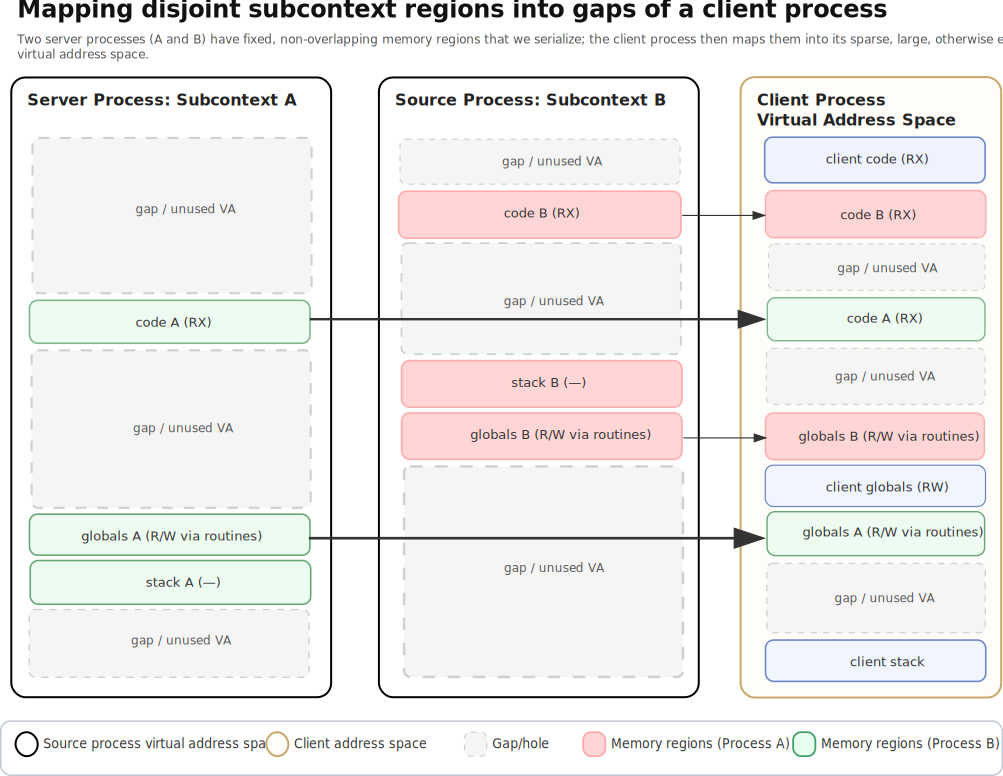
\includegraphics[width=\textwidth]{subcontexts_slotting_into_client.png}
    \caption{This is what the virtual address space of a client process looks like when it has mapped several subcontext.}
\end{figure}

\newpage
\section*{Architecture Overview}
\addcontentsline{toc}{section}{Architecture Overview}
The system is divided into three natural, primary roles: the \textbf{server-side library}, which is responsible for the creation of subcontexts; the 
\textbf{client-side library}, which maps and invokes subcontexts; and the \textbf{matchmaker}, which is part of the client library and enforces protections at runtime. This tripartite model emerged during prototyping in response to challenges around memory protection, control flow, and execution boundaries.

Initially, only the server and client roles were envisioned. The server generates image files, and the client loads and invokes them. However, ensuring memory safety required a third component: a runtime mediator that could enforce permissions during execution time and manage transitions. This mediator became the \textit{matchmaker}.

\subsection*{The Server-Side Library}
\addcontentsline{toc}{subsection}{The Server-Side Library}
The server-side library allows a process to serialize its own memory into an image file. This involves identifying relevant regions, reading their contents, and writing them into a structured binary file. Each serialized region is described in a header section that includes metadata such as the region’s starting address, size, permissions, and offset in the file. This metadata enables later reconstruction of the original memory layout during mapping by the client process, meaning that image files well-suited for reuse and distribution across processes.

\newpage
\subsubsection*{An Example Program}
The following program serializes its memory into an image file by picking up the methods provided by the server-side library.

\begin{ccode}
#include <stdio.h>
#include <stdlib.h>
#include "vm_sbc.h" // the header file for our system libraries

// the function to be serialized
void function1(int arg) {
	printf("Hello, world! arg=%d\n", arg);
}

int main(void) {
	// slot a pointer to the desired function into an array
	void (*funcs[1])(int) = { function1 };

	/* create_image_file is the library method which serializes
	 * and stores the snapshot of the memory of the process
	 */
	if (create_image_file(__FILE_NAME__, funcs, 1) != EXIT_SUCCESS) {
		fprintf(stderr, "Failed to create image file\n");
		return EXIT_FAILURE;
	}
}
\end{ccode}

\subsection*{The Client-Side Library}
\addcontentsline{toc}{subsection}{The Client-Side Library}
The client-side library supports mapping subcontext image files into memory and invoking their functionality. It uses the metadata in the image file to allocate a safe region in virtual memory, map each subcontext page with correct permissions, and link internal function pointers.

Once mapped, the client can invoke subcontext functions directly, treating the subcontext as a static, read-only module. The client is prohibited from modifying subcontext memory, and the subcontext has no access to client memory.

A global list of all mapped subcontexts is maintained by the matchmaker, which is a component of the client-side library which allows it to resolve which region of memory is active and to enforce protection boundaries dynamically.

\subsubsection*{An Example Program}
The following program maps an available image file into its memory as a subcontext via the client-side library and executes any available functions residing within the memory of the subcontext.

\begin{ccode}
#include <stdio.h>
#include <stdlib.h>
#include "vm_sbc.h" // the header file for our system libraries

int main(int argc, char **argv) {

	// check for the appropriate number of arguments
	if (argc < 2) {
		fprintf(stderr, "Usage: %s <img_file> [img_file...]\n", argv[0]);
		return EXIT_FAILURE;
	}

	/* init is a client-side library method that
	 * initializes both the matchmaker as well as 
	 * the entirety of the client-side library.
	 */
	init();

	int fds[MAX_IMG_FILES];
	size_t num_fds = 0;

	for (int i = 1; i < argc && num_fds < MAX_IMG_FILES; i++) {
		const char *img = argv[i] // the image file to map
		printf("Mapping image file: %s\n", img);

		/* map_subcontext is a client-side library method
		 * that maps the desired image file into the memory
		 * of the client process
		 */
		int fd = map_subcontext(img);
		if (fd < 0) {
			fprintf(stderr, "Failed to map %s\n", img);
			continue;
		}
		fds[num_fds++] = fd;

		int idx = 0;
		/* call_subcontext_function is a client-side
		 * library method which attempts to call a function
		 * residing in the memory of the mapped subcontext
		 */
		while (call_subcontext_function(idx, fd) == EXIT_SUCCESS) idx++;
		printf("Executed %d functions from %s\n", idx, img);

	}

	/* finalize is a client-side library method
	 * belonging to the matchmaker which disables
	 * all subcontext execute permissions and enables
	 * client execute permissions.
	 */
	finalize();
	return EXIT_SUCCESS;
}
\end{ccode}

This program begins by checking that the right number of arguments were provided by the user. The user should provide the names of image files they desire to map into the memory of the client process as subcontexts. They can provide up to \cinline{MAX_IMG_FILES} names of image files that exist.

The next step is to initialize the client-side library (which includes the matchmaker). This should always be done by user programs before attempting to utilize methods from the library. \cinline{init()} installs the segfault handler and ensures that the list of mapped subcontext and client memory regions are both zeroed out and prepared to account for any subcontexts which might presently be mapped in.

Next, the program enters a loop which maps the desired image files into its own memory (provided that they exist) as subcontexts and calls all functions available within the memory of the subcontext.

The program closes with a call to \cinline{finalize()}, which should always be called at the end of a user program, and should not be omitted. This method ensures that the matchmaker appropriately sets permissions--that all execute permissions for any mapped subcontexts are disabled and that the execute permissions for the client are enabled.

\subsection*{The Matchmaker}
\addcontentsline{toc}{subsection}{The Matchmaker}
The matchmaker is a runtime component that acts as a memory protection manager. It is part of the client-side library and ensures that when control flow enters a mapped subcontext, execution permissions are removed from the code regions of the client process and granted to those of the subcontext. When control returns to the client process, these permissions are reversed.

This toggling is implemented using page protection and signal trapping. When a client attempts to execute code in an unpermitted region, a \cinline{SIGSEGV} signal is triggered. The matchmaker intercepts the signal, inspects the instruction pointer, and adjusts page permissions accordingly before resuming execution.

This mechanism creates a well-defined entry point model: subcontext entry is only permitted at agreed-upon points, and all transitions are tightly controlled. The matchmaker enforces asymmetric visibility which means that clients know about subcontexts, but subcontexts remain unaware of the client process in which they are mapped or of other subcontexts.

We considered an alternative design where the matchmaker would itself be implemented as a subcontext, implicitly mapped into every client during initialization. However, this added unnecessary indirection. Embedding the matchmaker directly into the client library proved simpler and more robust.